\documentclass[11pt]{article}
\usepackage[utf8]{inputenc}	% Para caracteres en español
\usepackage{amsmath,amsthm,amsfonts,amssymb,amscd}
\usepackage{multirow,booktabs}
\usepackage[table]{xcolor}
\usepackage{fullpage}
\usepackage{lastpage}
\usepackage{enumitem}
\usepackage{fancyhdr}
\usepackage{mathrsfs}
\usepackage{wrapfig}
\usepackage{setspace}
\usepackage{calc}
\usepackage{multicol}
\usepackage{cancel}
\usepackage{float}
\usepackage{physics}
\usepackage[retainorgcmds]{IEEEtrantools}
\usepackage[margin=1cm]{geometry}
\usepackage{amsmath}
\newlength{\tabcont}
\setlength{\parindent}{0.0in}
\setlength{\parskip}{0.05in}
\usepackage{empheq}
\usepackage{framed}
\usepackage[most]{tcolorbox}
\usepackage{xcolor}
\usepackage[version=3]{mhchem}
\usepackage[english]{babel}
\usepackage[utf8]{inputenc}
\usepackage{graphicx}
\usepackage[colorinlistoftodos]{todonotes}

\colorlet{shadecolor}{orange!15}
\parindent 0in
\parskip 12pt
\geometry{margin=1in, headsep=0.25in}
\theoremstyle{definition}
\newtheorem{defn}{Definition}
\newtheorem{reg}{Rule}
\newtheorem{exer}{Exercise}
\newtheorem{note}{Note}
\begin{document}
\setcounter{section}{2}
%\setcounter{subsection}{}
\title{Problem Set 3}

%==============================================================
%\thispagestyle{empty}
\section*{}
\begin{center}
{\LARGE \bf Problem Set 3}\\
{\large Physics 180}\\
Olyn D. Desabelle
\end{center}

\begin{figure}[h!]
    \centering
    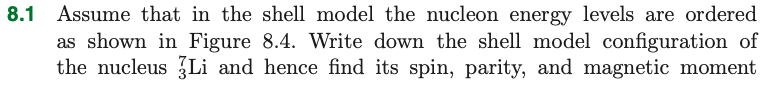
\includegraphics[scale = 0.5]{8.1a.png}
    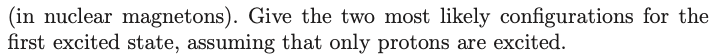
\includegraphics[scale = 0.5]{8.1b.png}
\end{figure}

\begin{figure}[h!]
    \centering
    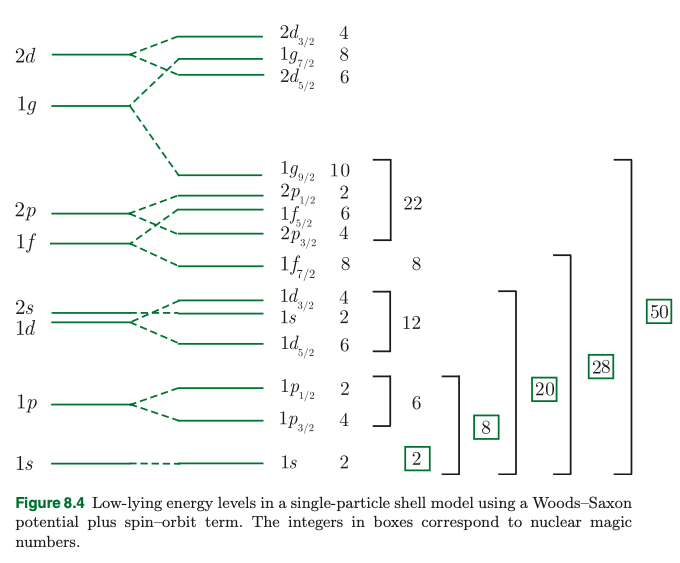
\includegraphics[scale = 0.5]{fig8.4.png}
\end{figure}

$_3^7$Li has $Z=3$ protons and $N = A-Z = 4$ neutrons (even-odd nuclei). From this, based on Figure 8.4, then we have the configurations:

\begin{align*}
    (1s_{1/2})^2(1p_{3/2})^1 \;\;\; \text{for protons}\\
    (1s_{1/2})^2(1p_{3/2})^2 \;\;\; \text{for neutrons}
\end{align*}

with all neutrons being paired, we only check the protons for contributions on spin, parity, and magnetic moment. We note that the protons have the following:

\begin{align*}
    j=3/2 \;\;\; l=1
\end{align*}

with no net spin contribution from then neutrons, then the total spin is:

\begin{equation}
\boxed{
    j=3/2
}
\end{equation}

its parity $P$ is then given by Equation 8.27:

\begin{align*}
    P = (-1)^l = -1^1
\end{align*}

\begin{equation}
\boxed{
    P = -1
}
\end{equation}

Its nuclear magnetic moment $\mu$ in nuclear magnetons is then given by Equation 8.28 and Equation 8.31 :

\begin{align*}
    \mu &= g_j j = j+2.3\\
    &= \frac{3}{2} + 2.3
\end{align*}

\begin{equation}
\boxed{
    \mu = 3.8 \; \text{nuclear magnetons}
}
\end{equation}

Assuming that only the protons are excited, then either the proton at $p_{3/2}$ gets excited to $p_{1/2}$, or a proton from $s_{1/2}$ gets excited to $p_{3/2}$, giving the following possible configurations:

\begin{equation}
\boxed{
    (1s_{1/2})^2(1p_{1/2})^1 \; \text{for protons} \;\;\; (1s_{1/2})^2(1p_{3/2})^2 \; \text{for neutrons}
}
\end{equation}

\begin{equation}
    \boxed{
        (1s_{1/2})^{1}(1p_{3/2})^2 \; \text{for protons} \;\;\; (1s_{1/2})^2(1p_{3/2})^2 \; \text{for neutrons}
    }
\end{equation}

\newpage
%==============================================================
\setcounter{equation}{0}
\begin{figure}[h!]
    \centering
    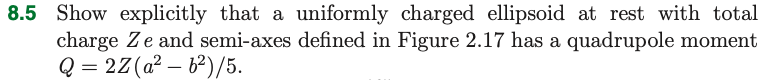
\includegraphics[scale = 0.55]{8.5.png}
\end{figure}

We begin with the equation for the quadrupole $Q$ given by Equation 8.32:

\begin{align*}
    eQ \equiv \int \rho(\mathbf{r}) (3z^2-r^2) d^3\mathbf{r} \tag*{(8.32)}\\
    Q = \frac{1}{e}\int \rho(\mathbf{r}) (3z^2-r^2) d^3\mathbf{r} \tag*{(8.32.1)}
\end{align*}

we then consider the given transformation:

\begin{figure}[h!]
    \centering
    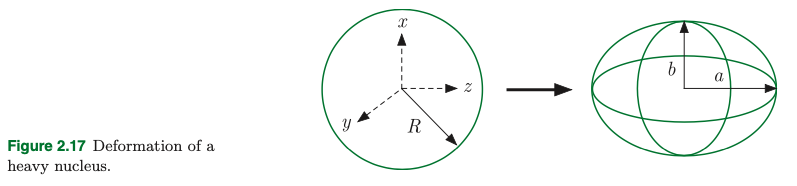
\includegraphics[scale = 0.55]{fig2.17.png}
\end{figure}

from the spherical model, we can express $r$ as:

\begin{align*}
    r^2 = x^2 + y^2 + z^2
\end{align*}

after the deformation to a prolate ellipsoid, $x,\; y,\; z$ become:

\begin{align*}
    x \to bx', \;\;\; y \to by', \;\;\; z \to az' \implies
    r^2 = b^2x'^2 + b^2y'^2 + a^2z'^2
\end{align*}

thus our quadrupole moment becomes:

\begin{align*}
    Q = \frac{1}{e}\int \int \int \rho(\mathbf{r}) (2a^2z'^2 - b^2x'^2 - b^2y'^2) \; dx'\; dy'\; dz' \tag*{(8.32.2)}
\end{align*}

we can rewrite the charge density $\rho(\mathbf{r})$ as the total charge over the volume, and with the given total charge $Ze$ we have:

\begin{align*}
    \rho(\mathbf{r}) &= \frac{Ze}{V}\\
                     &= \frac{Ze}{\frac{4}{3}\pi ab^2}\\
                    &= \frac{3Ze}{4\pi ab^2}
\end{align*}

and for the quadrupole moment we get:

\begin{align*}
    Q = \frac{3Z}{4\pi ab^2}\int \int \int (2a^2z'^2 - b^2x'^2 - b^2y'^2) \; dx'\; dy'\; dz' \tag*{(8.32.3)}
\end{align*}

we proceed to evaluate each integral term in spherical coordinates, noting the following change of variables:

\begin{align*}
    x' &\to s \cos\varphi \sin\theta \;\;\;\;\;\; 0\leq s \leq 1\\
    y' &\to s \sin\varphi \sin\theta \;\;\;\;\;\; 0\leq \varphi \leq \pi/2\\
    z' &\to s \cos\theta \;\;\;\;\;\;\;\;\;\;\;\;\;\; 0 \leq \theta \leq \pi/2  \\
    dx'dy'dz' &\to 8s^2 ab^2 \sin\theta ds d\varphi d\theta
\end{align*}

evaluating each integral, we have:

\begin{align*}
    \int \int \int 2a^2z'^2 \; dx'\; dy'\; dz' &= 2a^2 \int\int\int s^2 \cos^2\theta \; s^2 ab^2 \sin\theta\;  8ds d\varphi d\theta\\
    &= 16a^3 b^2 \int_{0}^{1}s^4\; ds \; \int_{0}^{\pi/2} \sin\theta \cos^2\theta \; d\theta \int_{0}^{\pi/2} d\varphi\\
    &= 16a^3 b^2 \left( \frac{1}{5} \right) \left(\frac{1}{3}\right) \left(\frac{\pi}{2}\right)\\
    &= 8a^3 b^2\frac{\pi}{15}
 \end{align*}

\begin{align*}
    \int\int\int b^2x'^2 \; dx'\; dy'\; dz' &= b^2 \int\int\int s^2\cos^2\varphi \sin^2\theta \; s^2 ab^2 \sin\theta\;  8ds d\varphi d\theta\\
    &= 8ab^4 \int_{0}^{1}s^4\; ds \;  \int_{0}^{\pi/2} \cos^2\varphi \; d\varphi \int_{0}^{\pi/2} \sin^3\theta \; d\theta\\
    &= 8ab^4 \left(\frac{1}{5}\right) \left(\frac{\pi}{4}\right) \left(\frac{2}{3}\right)\\
    &= 8ab^4 \frac{\pi}{30}
\end{align*}

\begin{align*}
    \int\int\int b^2y'^2 \; dx'\; dy'\; dz' &= b^2 \int\int\int s^2\sin^2\varphi \sin^2\theta \; s^2 ab^2 \sin\theta \; 8ds d\varphi d\theta\\
    &= 8ab^4 \int_{0}^{1}s^4\; ds \;  \int_{0}^{\pi/2} \sin^2\varphi \; d\varphi \int_{0}^{\pi/2} \sin^3\theta \; d\theta\\
    &= 8ab^4 \left(\frac{1}{5}\right) \left(\frac{\pi}{4}\right) \left(\frac{2}{3}\right)\\
    &= 8ab^4 \frac{\pi}{30}
\end{align*}

thus we have:

\begin{align*}
    Q = \frac{3Z}{4\pi ab^2} \left(8a^3 b^2\frac{\pi}{15} - 8ab^4 \frac{\pi}{15} \right)
\end{align*}

\begin{equation}
\boxed{
    Q = \frac{2Z(a^2-b^2)}{5}
}
\end{equation}

\end{document}